% Template for PLoS
% Version 3.5 March 2018
%
% % % % % % % % % % % % % % % % % % % % % %
%
% -- IMPORTANT NOTE
%
% This template contains comments intended
% to minimize problems and delays during our production
% process. Please follow the template instructions
% whenever possible.
%
% % % % % % % % % % % % % % % % % % % % % % %
%
% Once your paper is accepted for publication,
% PLEASE REMOVE ALL TRACKED CHANGES in this file
% and leave only the final text of your manuscript.
% PLOS recommends the use of latexdiff to track changes during review, as this will help to maintain a clean tex file.
% Visit https://www.ctan.org/pkg/latexdiff?lang=en for info or contact us at latex@plos.org.
%
%
% There are no restrictions on package use within the LaTeX files except that
% no packages listed in the template may be deleted.
%
% Please do not include colors or graphics in the text.
%
% The manuscript LaTeX source should be contained within a single file (do not use \input, \externaldocument, or similar commands).
%
% % % % % % % % % % % % % % % % % % % % % % %
%
% -- FIGURES AND TABLES
%
% Please include tables/figure captions directly after the paragraph where they are first cited in the text.
%
% DO NOT INCLUDE GRAPHICS IN YOUR MANUSCRIPT
% - Figures should be uploaded separately from your manuscript file.
% - Figures generated using LaTeX should be extracted and removed from the PDF before submission.
% - Figures containing multiple panels/subfigures must be combined into one image file before submission.
% For figure citations, please use "Fig" instead of "Figure".
% See http://journals.plos.org/plosone/s/figures for PLOS figure guidelines.
%
% Tables should be cell-based and may not contain:
% - spacing/line breaks within cells to alter layout or alignment
% - do not nest tabular environments (no tabular environments within tabular environments)
% - no graphics or colored text (cell background color/shading OK)
% See http://journals.plos.org/plosone/s/tables for table guidelines.
%
% For tables that exceed the width of the text column, use the adjustwidth environment as illustrated in the example table in text below.
%
% % % % % % % % % % % % % % % % % % % % % % % %
%
% -- EQUATIONS, MATH SYMBOLS, SUBSCRIPTS, AND SUPERSCRIPTS
%
% IMPORTANT
% Below are a few tips to help format your equations and other special characters according to our specifications. For more tips to help reduce the possibility of formatting errors during conversion, please see our LaTeX guidelines at http://journals.plos.org/plosone/s/latex
%
% For inline equations, please be sure to include all portions of an equation in the math environment.  For example, x$^2$ is incorrect; this should be formatted as $x^2$ (or $\mathrm{x}^2$ if the romanized font is desired).
%
% Do not include text that is not math in the math environment. For example, CO2 should be written as CO\textsubscript{2} instead of CO$_2$.
%
% Please add line breaks to long display equations when possible in order to fit size of the column.
%
% For inline equations, please do not include punctuation (commas, etc) within the math environment unless this is part of the equation.
%
% When adding superscript or subscripts outside of brackets/braces, please group using {}.  For example, change "[U(D,E,\gamma)]^2" to "{[U(D,E,\gamma)]}^2".
%
% Do not use \cal for caligraphic font.  Instead, use \mathcal{}
%
% % % % % % % % % % % % % % % % % % % % % % % %
%
% Please contact latex@plos.org with any questions.
%
% % % % % % % % % % % % % % % % % % % % % % % %

\documentclass[10pt,letterpaper]{article}
\usepackage[top=0.85in,left=2.75in,footskip=0.75in]{geometry}

% amsmath and amssymb packages, useful for mathematical formulas and symbols
\usepackage{amsmath,amssymb}

% Use adjustwidth environment to exceed column width (see example table in text)
\usepackage{changepage}

% Use Unicode characters when possible
\usepackage[utf8x]{inputenc}

% textcomp package and marvosym package for additional characters
\usepackage{textcomp,marvosym}

% cite package, to clean up citations in the main text. Do not remove.
\usepackage{cite}

% Use nameref to cite supporting information files (see Supporting Information section for more info)
\usepackage{nameref,hyperref}

% line numbers
\usepackage[right]{lineno}

% Packages included by the papers authors
\usepackage[capitalize]{cleveref}
\usepackage{float}

\usepackage{verbatim}

\usepackage{listings}
\IfFileExists{zi4.sty}{\usepackage{zi4}}{\usepackage{inconsolata}} % 'Inconsolata' is my monospace font of choice
\lstset{
  columns=flexible,
  keepspaces=true,
  basicstyle=\ttfamily,
  extendedchars=true,
  showspaces=false,
  showtabs=false,
  showstringspaces=false,
  frame=single,
  captionpos=b,
}

% ligatures disabled
\usepackage{microtype}
\DisableLigatures[f]{encoding = *, family = * }

% color can be used to apply background shading to table cells only
\usepackage[table]{xcolor}

% array package and thick rules for tables
\usepackage{array}

% create "+" rule type for thick vertical lines
\newcolumntype{+}{!{\vrule width 2pt}}

% create \thickcline for thick horizontal lines of variable length
\newlength\savedwidth
\newcommand\thickcline[1]{%
  \noalign{\global\savedwidth\arrayrulewidth\global\arrayrulewidth 2pt}%
  \cline{#1}%
  \noalign{\vskip\arrayrulewidth}%
  \noalign{\global\arrayrulewidth\savedwidth}%
}

% \thickhline command for thick horizontal lines that span the table
\newcommand\thickhline{\noalign{\global\savedwidth\arrayrulewidth\global\arrayrulewidth 2pt}%
\hline
\noalign{\global\arrayrulewidth\savedwidth}}


% Remove comment for double spacing
%\usepackage{setspace}
%\doublespacing

% Text layout
\raggedright
\setlength{\parindent}{0.5cm}
\textwidth 5.25in
\textheight 8.75in

% Bold the 'Figure #' in the caption and separate it from the title/caption with a period
% Captions will be left justified
\usepackage[aboveskip=1pt,labelfont=bf,labelsep=period,justification=raggedright,singlelinecheck=off]{caption}
\renewcommand{\figurename}{Fig}

% Use the PLoS provided BiBTeX style
\bibliographystyle{plos2015}

% Remove brackets from numbering in List of References
\makeatletter
\renewcommand{\@biblabel}[1]{\quad#1.}
\makeatother



% Header and Footer with logo
\usepackage{lastpage,fancyhdr,graphicx}
\usepackage[outdir=build/]{epstopdf}
%\pagestyle{myheadings}
\pagestyle{fancy}
\fancyhf{}
%\setlength{\headheight}{27.023pt}
%\lhead{\includegraphics[width=2.0in]{PLOS-submission.eps}}
\rfoot{\thepage/\pageref{LastPage}}
\renewcommand{\headrulewidth}{0pt}
\renewcommand{\footrule}{\hrule height 2pt \vspace{2mm}}
\fancyheadoffset[L]{2.25in}
\fancyfootoffset[L]{2.25in}
\lfoot{\today}

%% Include all macros below

\newcommand{\lorem}{{\bf LOREM}}
\newcommand{\ipsum}{{\bf IPSUM}}

\newcommand{\code}[1]{\texttt{#1}}

%% END MACROS SECTION


\begin{document}
  \vspace*{0.2in}
  \begin{flushleft}
    % Title must be 250 characters or less.
{\Large
% Please use "sentence case" for title and headings (capitalize only the first word in a title
\textbf\newline{Title of submission to PLOS journals}
}
\newline

    % Insert author names, affiliations and corresponding author email (do not include titles, positions, or degrees).
\\
Name1 Surname\textsuperscript{1,2\Yinyang},
Name2 Surname\textsuperscript{2\Yinyang},
Name3 Surname\textsuperscript{2,3\textcurrency},
Name4 Surname\textsuperscript{2},
Name5 Surname\textsuperscript{2\ddag},
Name6 Surname\textsuperscript{2\ddag},
Name7 Surname\textsuperscript{1,2,3*},
with the Lorem Ipsum Consortium\textsuperscript{\textpilcrow}
\\
\bigskip
\textbf{1} Affiliation Dept/Program/Center, Institution Name, City, State, Country
\\
\textbf{2} Affiliation Dept/Program/Center, Institution Name, City, State, Country
\\
\textbf{3} Affiliation Dept/Program/Center, Institution Name, City, State, Country
\\
\bigskip

% Insert additional author notes using the symbols described below. Insert symbol callouts after author names as necessary.
%
% Remove or comment out the author notes below if they aren't used.
%
% Primary Equal Contribution Note
\Yinyang These authors contributed equally to this work.

% Additional Equal Contribution Note
% Also use this double-dagger symbol for special authorship notes, such as senior authorship.
\ddag These authors also contributed equally to this work.

% Current address notes
\textcurrency Current Address: Dept/Program/Center, Institution Name, City, State, Country % change symbol to "\textcurrency a" if more than one current address note
% \textcurrency b Insert second current address
% \textcurrency c Insert third current address

% Deceased author note
\dag Deceased

% Group/Consortium Author Note
\textpilcrow Membership list can be found in the Acknowledgments section.

% Use the asterisk to denote corresponding authorship and provide email address in note below.
* correspondingauthor@institute.edu

  \end{flushleft}
  % Please keep the abstract below 300 words
\section*{Abstract}
Lorem ipsum dolor sit amet, consectetur adipiscing elit. Curabitur eget porta erat. Morbi consectetur est vel gravida pretium. Suspendisse ut dui eu ante cursus gravida non sed sem. Nullam sapien tellus, commodo id velit id, eleifend volutpat quam. Phasellus mauris velit, dapibus finibus elementum vel, pulvinar non tellus. Nunc pellentesque pretium diam, quis maximus dolor faucibus id. Nunc convallis sodales ante, ut ullamcorper est egestas vitae. Nam sit amet enim ultrices, ultrices elit pulvinar, volutpat risus.


  \linenumbers

  \section*{Introduction}

\finishsection

  \section*{Materials and methods}
\subsection*{Etiam eget sapien nibh}

% For figure citations, please use "Fig" instead of "Figure".
% Nulla mi mi, Fig~\ref{fig1} venenatis sed ipsum varius, volutpat euismod diam.
Proin rutrum vel massa non gravida. Quisque tempor sem et dignissim rutrum. Lorem ipsum dolor sit amet, consectetur adipiscing elit. Morbi at justo vitae nulla elementum commodo eu id massa. In vitae diam ac augue semper tincidunt eu ut eros. Fusce fringilla erat porttitor lectus cursus, \nameref{S1_Video} vel sagittis arcu lobortis. Aliquam in enim semper, aliquam massa id, cursus neque. Praesent faucibus semper libero.

% Place figure captions after the first paragraph in which they are cited.
% \begin{figure}[!h]
% \caption{{\bf Bold the figure title.}
% Figure caption text here, please use this space for the figure panel descriptions instead of using subfigure commands. A: Lorem ipsum dolor sit amet. B: Consectetur adipiscing elit.}
% \label{fig1}
% \end{figure}

  % Results and Discussion can be combined.
\section*{Results}
Nulla mi mi, venenatis sed ipsum varius, Table~\ref{table1} volutpat euismod diam. Proin rutrum vel massa non gravida. Quisque tempor sem et dignissim rutrum. Lorem ipsum dolor sit amet, consectetur adipiscing elit. Morbi at justo vitae nulla elementum commodo eu id massa. In vitae diam ac augue semper tincidunt eu ut eros. Fusce fringilla erat porttitor lectus cursus, vel sagittis arcu lobortis. Aliquam in enim semper, aliquam massa id, cursus neque. Praesent faucibus semper libero.

% Place tables after the first paragraph in which they are cited.
\begin{table}[!ht]
\begin{adjustwidth}{-2.25in}{0in} % Comment out/remove adjustwidth environment if table fits in text column.
\centering
\caption{
{\bf Table caption Nulla mi mi, venenatis sed ipsum varius, volutpat euismod diam.}}
\begin{tabular}{|l+l|l|l|l|l|l|l|}
\hline
\multicolumn{4}{|l|}{\bf Heading1} & \multicolumn{4}{|l|}{\bf Heading2}\\ \thickhline
$cell1 row1$ & cell2 row 1 & cell3 row 1 & cell4 row 1 & cell5 row 1 & cell6 row 1 & cell7 row 1 & cell8 row 1\\ \hline
$cell1 row2$ & cell2 row 2 & cell3 row 2 & cell4 row 2 & cell5 row 2 & cell6 row 2 & cell7 row 2 & cell8 row 2\\ \hline
$cell1 row3$ & cell2 row 3 & cell3 row 3 & cell4 row 3 & cell5 row 3 & cell6 row 3 & cell7 row 3 & cell8 row 3\\ \hline
\end{tabular}
\begin{flushleft} Table notes Phasellus venenatis, tortor nec vestibulum mattis, massa tortor interdum felis, nec pellentesque metus tortor nec nisl. Ut ornare mauris tellus, vel dapibus arcu suscipit sed.
\end{flushleft}
\label{table1}
\end{adjustwidth}
\end{table}


%PLOS does not support heading levels beyond the 3rd (no 4th level headings).
\subsection*{\lorem\ and \ipsum\ nunc blandit a tortor}
\subsubsection*{3rd level heading}
Maecenas convallis mauris sit amet sem ultrices gravida. Etiam eget sapien nibh. Sed ac ipsum eget enim egestas ullamcorper nec euismod ligula. Curabitur fringilla pulvinar lectus consectetur pellentesque. Quisque augue sem, tincidunt sit amet feugiat eget, ullamcorper sed velit. Sed non aliquet felis. Lorem ipsum dolor sit amet, consectetur adipiscing elit. Mauris commodo justo ac dui pretium imperdiet. Sed suscipit iaculis mi at feugiat.

\begin{enumerate}
	\item{react}
	\item{diffuse free particles}
	\item{increment time by dt and go to 1}
\end{enumerate}


\subsection*{Sed ac quam id nisi malesuada congue}

Nulla mi mi, venenatis sed ipsum varius, volutpat euismod diam. Proin rutrum vel massa non gravida. Quisque tempor sem et dignissim rutrum. Lorem ipsum dolor sit amet, consectetur adipiscing elit. Morbi at justo vitae nulla elementum commodo eu id massa. In vitae diam ac augue semper tincidunt eu ut eros. Fusce fringilla erat porttitor lectus cursus, vel sagittis arcu lobortis. Aliquam in enim semper, aliquam massa id, cursus neque. Praesent faucibus semper libero.

\begin{itemize}
	\item First bulleted item.
	\item Second bulleted item.
	\item Third bulleted item.
\end{itemize}

  \section*{Discussion}

\finishsection

  \section*{Conclusion}

CO\textsubscript{2} Maecenas convallis mauris sit amet sem ultrices gravida. Etiam eget sapien nibh. Sed ac ipsum eget enim egestas ullamcorper nec euismod ligula. Curabitur fringilla pulvinar lectus consectetur pellentesque. Quisque augue sem, tincidunt sit amet feugiat eget, ullamcorper sed velit.

Sed non aliquet felis. Lorem ipsum dolor sit amet, consectetur adipiscing elit. Mauris commodo justo ac dui pretium imperdiet. Sed suscipit iaculis mi at feugiat. Ut neque ipsum, luctus id lacus ut, laoreet scelerisque urna. Phasellus venenatis, tortor nec vestibulum mattis, massa tortor interdum felis, nec pellentesque metus tortor nec nisl. Ut ornare mauris tellus, vel dapibus arcu suscipit sed. Nam condimentum sem eget mollis euismod. Nullam dui urna, gravida venenatis dui et, tincidunt sodales ex. Nunc est dui, sodales sed mauris nec, auctor sagittis leo. Aliquam tincidunt, ex in facilisis elementum, libero lectus luctus est, non vulputate nisl augue at dolor.

  \section*{Project \code{latex2plos}}

The latex2plos project \cite{latex2plos} is a Python \cite{Python} powered library/console tool for automated preparation of your \LaTeX~paper for submission in PLOS journals, and is at the core of the proposed automated workflow.
It's designed to address the issues discussed in the "Introduction" section, and resolve them effectively.
It does so by taking the original \LaTeX~manuscript as its input, transforming the said manuscript and its resources (such as figures, reference information, and code listings) into a submission-ready version of the paper, that conforms to the official PLOS figure and \LaTeX~guidelines \cite{PLOS:Figures, PLOS:LaTeX}.
For greater transparency the source code of the latex2plos project \cite{latex2plos} has been publicly released under an OSI approved BSD Open Source license \cite{OSI:BSD}, right from \emph{day one} of its creation.

The latex2plos project is composed of three distinct components: a \LaTeX~parser, transformers and console shell interface.

The \LaTeX~parser is based on regular expressions.
For each line of input the parser first checks if it starts with a commented-out \LaTeX~command, and if not it then looks for characteristic markers that match against a specific transformer.
If no such marker is found the line is copied as-is, otherwise an appropriate transformer is invoked where it's able to manipulate the \LaTeX~document directly and/or its referenced resources.
The document itself is processed and streamed through on the fly, for maximum efficiency.

Transformers manipulate the \LaTeX~document and its referenced resources (such as figures, reference information, and code listings), to achieve compliance with the official PLOS figure and \LaTeX~guidelines \cite{PLOS:Figures, PLOS:LaTeX}.
All transformers are implemented as plugins.
The dynamic plugin subsystem, based on the \code{simple\_plugins} project \cite{Project:simple_plugins:CodeRepository}, provides automatic transformer plugin discovery and registration.

The author of this paper is a firm believer in the API-centric software development doctrine and, like most of his other Open Source projects, latex2plos is first and foremost a Python library -- with its public API exposed through a console shell interface as well.

This remainder of this section has been carried over from the template4plos project \cite{template4plos}, to demonstrate the commonly used \LaTeX~features that are not present in the original PLOS \LaTeX~template, and verify that the latex2plos project is able to handle them properly.
While doing that, it also documents the individual transformer plugins.

\subsection*{\code{verbatiminput}}

\code{latex2plos.transformers.VerbatimInputTransformer} will transform a \verb|\verbatiminput| file inclusion into its equivalent \verb|\begin{verbatim}...\end{verbatim}| call, as in the example below \cite{Project:friendly_name_mixin:CodeRepository}:

\verbatiminput{listings/friendly_name_mixin.py}

\subsection*{\code{bibliography}}

\code{latex2plos.transformers.BibliographyTransformer} will transform a \verb|\bibliography| file inclusion into its equivalent \verb|\begin{thebibliography}...\end{thebibliography}| call, as demonstrated by this paper (\code{paper.tex}) and its BiBTeX database (\code{references.bib}).

This is done as PLOS does not allow submission of BiBTeX databases, and instead requires the reference information to be embedded in the paper directly \cite{PLOS:LaTeX}.

\subsection*{\code{lstinputlisting}}

\code{latex2plos.transformers.InputListingTransformer} will copy over the files referenced by \verb|\lstinputlisting| into the papers export directory, as in the examples below:

\lstinputlisting[language=Python,caption={\code{friendly\_name\_mixin} project source code \cite{Project:friendly_name_mixin:CodeRepository}}]{listings/friendly_name_mixin.py}

\lstinputlisting[language=Python,caption={\code{friendly\_name\_mixin} project unit tests \cite{Project:friendly_name_mixin:CodeRepository}}]{listings/tests.py}

\pagebreak
\subsection*{\code{includegraphics}}

\code{latex2plos.transformers.IncludeGraphicsTransformer} will copy over the figures referenced by \verb|\includegraphics| into the papers export directory, as shown in \cref{fig:petar-avatar,fig:3-clamped-free-beam-decimal-precision-errors,fig:barbero-viscoelastic-natural-frequencies,fig:barbero-viscoelastic-damage-analysis}.
It will also transform all figures into the TIFF image format (LZW compression, at 300 dpi) and remove/comment-out them from the papers exported PDF, as per PLOS requirements \cite{PLOS:LaTeX, PLOS:Figures}.

\begin{figure}[H]
    \centering
    
\includegraphics[height=6cm]{figures/petar-gravatar.png}
    \caption{Petar Marić gravatar (PNG image format) \cite{Maric:Gravatar}}
    \label{fig:petar-avatar}
\end{figure}

\begin{figure}[H]
    \centering
    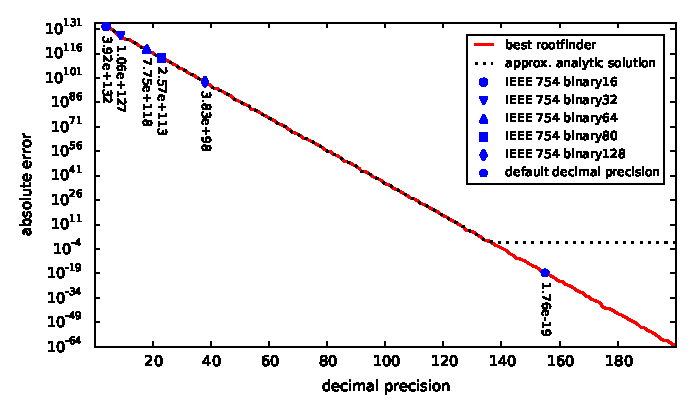
\includegraphics[width=\linewidth]{figures/decimal-precision-error@3-clamped-free-beam.eps}
    \caption{Maximum root-finding errors (across all 100 modes) of clamped-free beam's (LJ=3) characteristic function (EPS image format) \cite{Maric:2017}}
    \label{fig:3-clamped-free-beam-decimal-precision-errors}
\end{figure}

\begin{figure}[H]
    \centering
    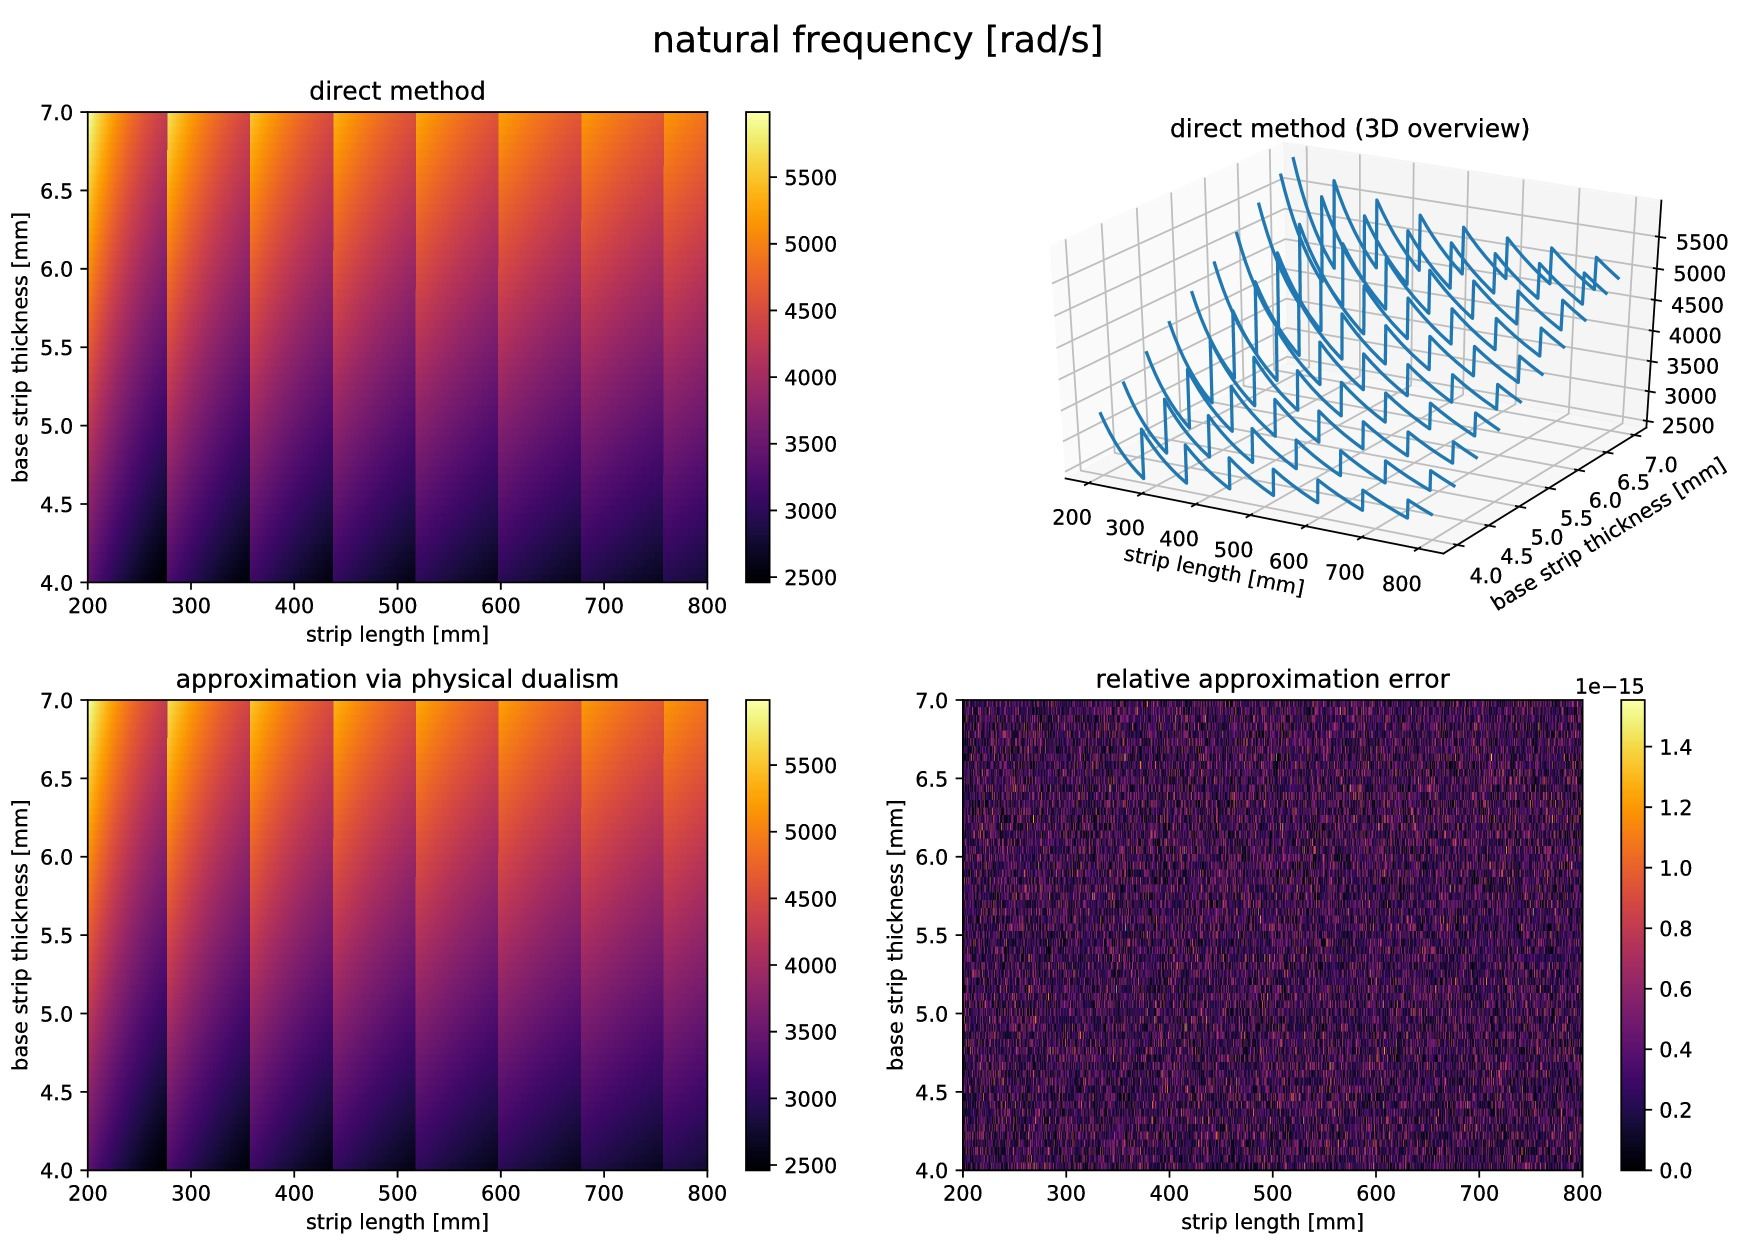
\includegraphics[width=\linewidth]{figures/barbero-viscoelastic@local-p1.jpg}
    \caption{Viscoelastic natural frequencies (JPEG image format) \cite{Milasinovic:2018}}
    \label{fig:barbero-viscoelastic-natural-frequencies}
\end{figure}

\begin{figure}[H]
    \centering
    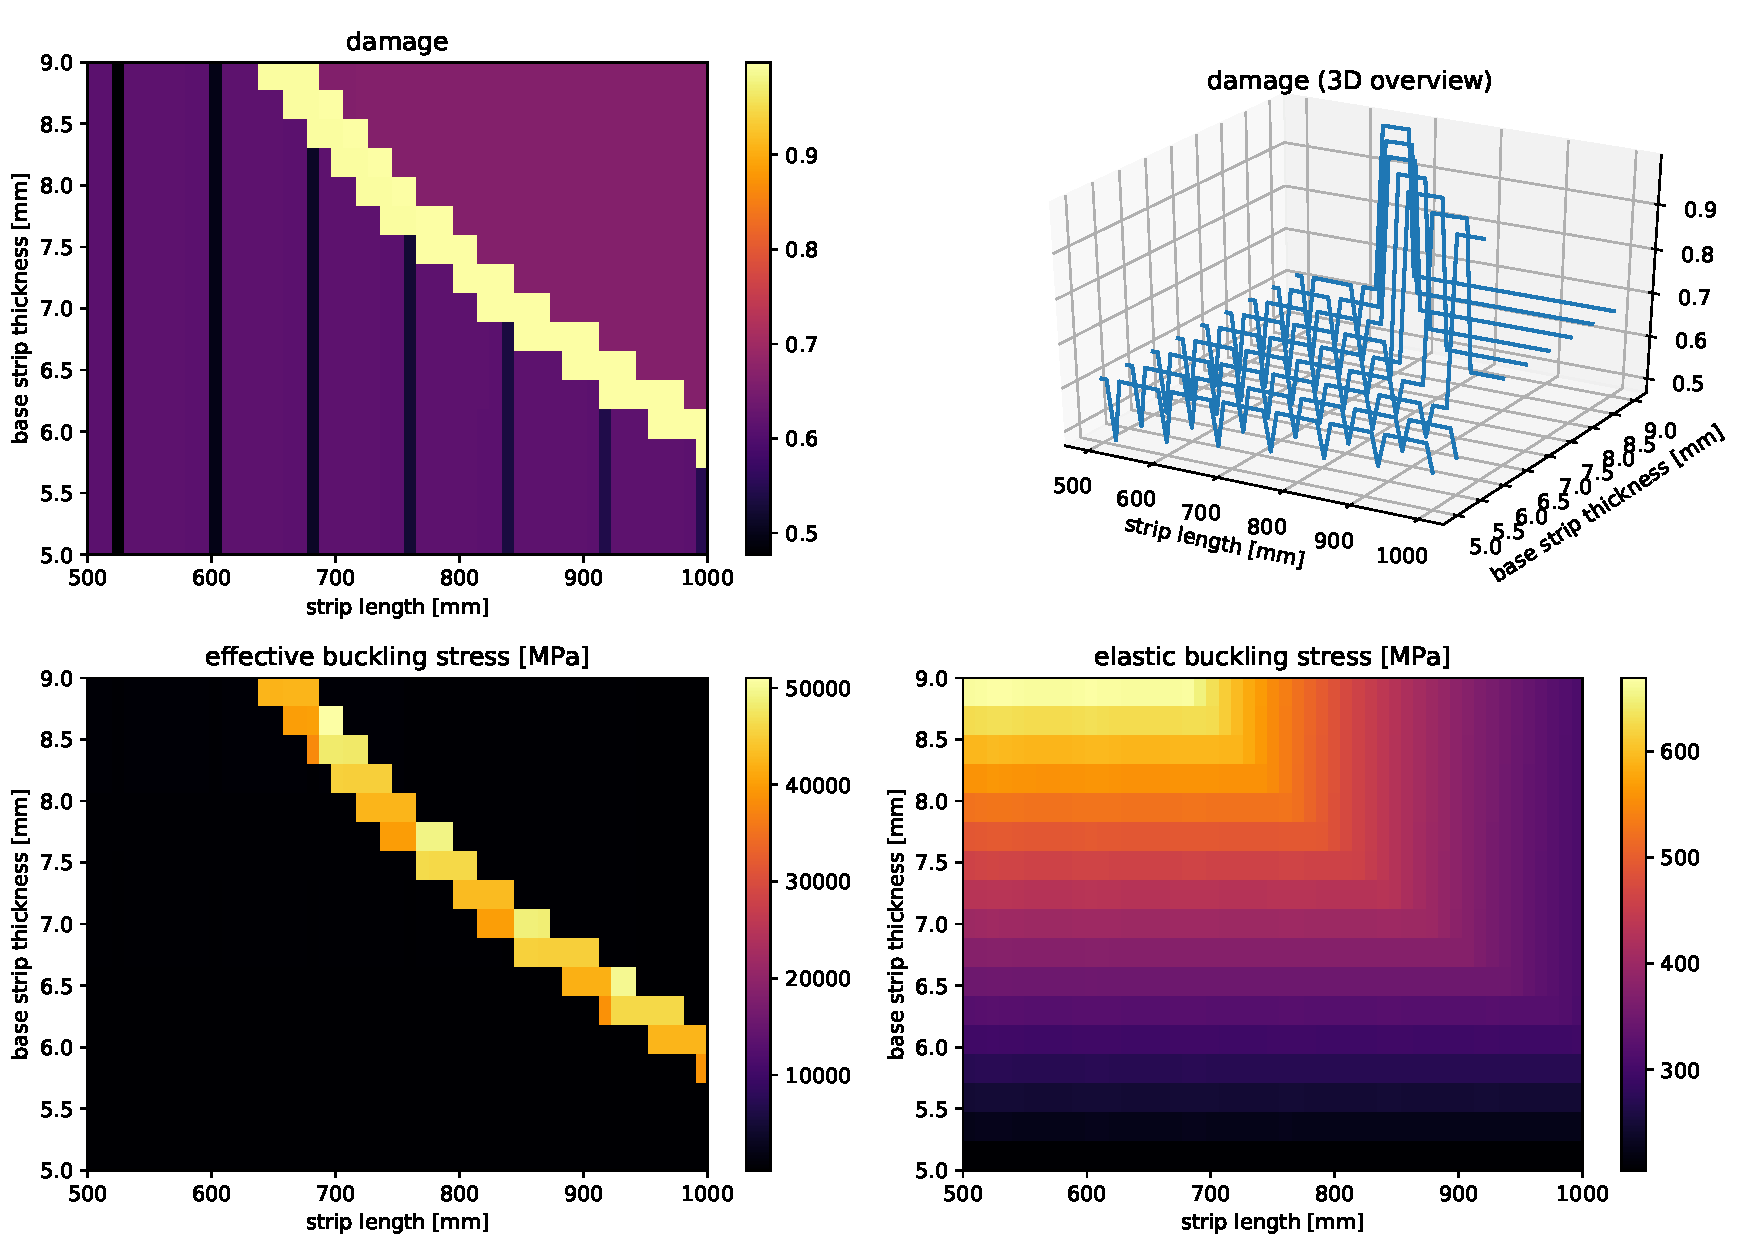
\includegraphics[width=\linewidth]{figures/barbero-viscoelastic@fsm-damage-analysis.pdf}
    \caption{\code{fsm\_damage\_analysis} project example experiment report (PDF image format) \cite{Project:fsm_damage_analysis:CodeRepository}}
    \label{fig:barbero-viscoelastic-damage-analysis}
\end{figure}

\subsection*{Multiple \LaTeX~files workflow}

\code{latex2plos.transformers.IncludeTransformer} will embed the contents of files referenced by \verb|\include| into the exported paper directly, whereas \code{latex2plos.transformers.InputTransformer} will do the same for \verb|\input|, as demonstrated by this paper (\code{paper.tex}) and its referenced \code{.tex} files (\code{preamble.tex},  \code{head/*.tex} and \code{sections/*.tex}).

This is done as PLOS does not allow submission of multiple \code{.tex} files, and instead requires them to be combined into a single, cohesive \code{.tex} file \cite{PLOS:LaTeX}.

  \section*{Supporting information}

% Include only the SI item label in the paragraph heading. Use the \nameref{label} command to cite SI items in the text.
\paragraph*{S1 Fig.}
\label{S1_Fig}
{\bf Bold the title sentence.} Add descriptive text after the title of the item (optional).

\paragraph*{S2 Fig.}
\label{S2_Fig}
{\bf Lorem ipsum.} Maecenas convallis mauris sit amet sem ultrices gravida. Etiam eget sapien nibh. Sed ac ipsum eget enim egestas ullamcorper nec euismod ligula. Curabitur fringilla pulvinar lectus consectetur pellentesque.

\paragraph*{S1 File.}
\label{S1_File}
{\bf Lorem ipsum.}  Maecenas convallis mauris sit amet sem ultrices gravida. Etiam eget sapien nibh. Sed ac ipsum eget enim egestas ullamcorper nec euismod ligula. Curabitur fringilla pulvinar lectus consectetur pellentesque.

\paragraph*{S1 Video.}
\label{S1_Video}
{\bf Lorem ipsum.}  Maecenas convallis mauris sit amet sem ultrices gravida. Etiam eget sapien nibh. Sed ac ipsum eget enim egestas ullamcorper nec euismod ligula. Curabitur fringilla pulvinar lectus consectetur pellentesque.

\paragraph*{S1 Appendix.}
\label{S1_Appendix}
{\bf Lorem ipsum.} Maecenas convallis mauris sit amet sem ultrices gravida. Etiam eget sapien nibh. Sed ac ipsum eget enim egestas ullamcorper nec euismod ligula. Curabitur fringilla pulvinar lectus consectetur pellentesque.

\paragraph*{S1 Table.}
\label{S1_Table}
{\bf Lorem ipsum.} Maecenas convallis mauris sit amet sem ultrices gravida. Etiam eget sapien nibh. Sed ac ipsum eget enim egestas ullamcorper nec euismod ligula. Curabitur fringilla pulvinar lectus consectetur pellentesque.

  \section*{Acknowledgments}

\finishsection

The work reported in this paper is a part of the investigation within the research project \ldots

We would also like to thank the Open Source community for the projects that helped create this paper: \LaTeX \cite{LaTeX}, Python \cite{Python}, latex2plos \cite{latex2plos} and template4plos \cite{template4plos}.


  \nolinenumbers

  % Either type in your references using
  % \begin{thebibliography}{}
  % \bibitem{}
  % Text
  % \end{thebibliography}
  %
  % or
  %
  % Compile your BiBTeX database using our plos2015.bst
  % style file and paste the contents of your .bbl file
  % here. See http://journals.plos.org/plosone/s/latex for
  % step-by-step instructions.
  \bibliography{references}
\end{document}
